\section{Unsupervised Learning - Clustering}
What we have seen so far are all examples of \textbf{supervised learning}, which required a labeled dataset to learn from. This process
is usually extremely expensive and it could happen that we don't have access to labeled data at all. 
\\In such cases, we can resort to \textbf{unsupervised learning} techniques, which can be used to group data points into \textbf{clusters}. 

\subsection{K-Means Clustering}
One of the most popular clustering algorithms is \textbf{K-Means Clustering}. The setting is the following:
\begin{itemize}
    \item We have a dataset of $n$ points $\{x_1, x_2, \ldots, x_n\}$ in $\mathbb{R}^d$.
    \item We assume that examples should be grouped into $k$ clusters, we will see later how to choose $k$;
    \item Each cluster $i$ is represented by its \textbf{centroid} (mean) $\mu_i$;
\end{itemize}
\subsubsection*{Algorithm}
The K-Means algorithm works as follows:
\begin{enumerate}
    \item Initialize $k$ cluster means $\mu_1, \mu_2, \ldots, \mu_k$ (randomly or using some heuristic);
    \item Repeat until convergence:
    \begin{itemize}
        \item \textbf{Assignment step}: Assign each point $x_j$ to the nearest cluster mean;
        \item \textbf{Update step}: Update cluster means according to the assigned points;
    \end{itemize}
\end{enumerate}
The algorithm converges when the assignments no longer change or the cluster means stabilize. 
\subsubsection*{Distance Metrics}
To compute the distance between points and cluster means, we have to choose a distance metric, the most common choices are:
\begin{itemize}
    \item Euclidean distance in $\mathbb{R}^d$;
    \[d(\boldsymbol{x}, \boldsymbol{x}') = \sqrt{\sum_{i=1}^d (x_i - x_i')^2}\]
    \item Manhattan distance:
    \[d(\boldsymbol{x}, \boldsymbol{x}') = \sum_{i=1}^d |x_i - x_i'|\]
    \item Cosine similarity:
    \[d(\boldsymbol{x}, \boldsymbol{x}') = 1 - \frac{\boldsymbol{x}^T  \boldsymbol{x}'}{||\boldsymbol{x}|| \, ||\boldsymbol{x}'||}\]
\end{itemize}
\subsection{Quality of Clustering}
Since we are working in an unsupervised setting, we don't have labels to evaluate the quality of our clustering. However, we can define the following metrics:
\defib{Sum-of-Squared error criterion}
{
    The sum-of-squared error criterion is defined as:
    \begin{itemize}
        \item let $n_i$ be the number of points assigned to cluster $i$ ($D_i$);
        \item let $\mu_i$ be the centroid of cluster $i$. It can be computed as:
        \[\mu_i = \frac{1}{n_i} \sum_{\boldsymbol{x} \in D_i} \boldsymbol{x}\]
        \item the sum-of-squared error criterion is defined as:
        \[ E = \sum_{i=1}^k \sum_{\boldsymbol{x} \in D_i} ||\boldsymbol{x} - \mu_i||^2 \]
    \end{itemize}
    It measures the squared error incurred in representing each point by its cluster centroid.
}
\subsection{Gaussian Mixture Models (GMM)}
The idea behind Gaussian Mixture Models is to model the data as a mixture of several Gaussian distributions. 
Each cluster is represented by a Gaussian distribution with its own parameters (mean and covariance).
It assumes that the number of clusters $K$ is given and that each data point is generated from one of the $K$ Gaussian distributions.
\subsubsection*{Parameter Estimation}
If we wanted to estimate the parameters of the Gaussians (means and covariances), we could use Maximum Log-Likelihood Estimation (MLE).
\[ \theta^* = \arg \max_{\theta} \mathcal{L}(\theta|\mathcal{D})\]
where $\theta$ are the parameters of the Gaussians and $\mathcal{D}$ is the dataset.
\[ \mathcal{L}(\theta|\mathcal{D}) = \sum_{i=1}^{n} \log \left( \sum_{h = 1}^{K}p(x_i | \theta_k) \right) \]
However, MLE cannot be used directly, since the cluster assignments are unknown.
Instead, we can apply an iterative approach called the \textbf{Expectation-Maximization (EM)}.

\subsubsection*{Expectation-Maximization (EM) Algorithm}
The EM algorithm consists of two main steps:
\begin{enumerate}
    \item \textbf{E-step (Expectation step)}: Compute the expected cluster assignments given the current parameters;
    \item \textbf{M-step (Maximization step)}: Update the parameters of the Gaussians given the expected cluster assignments;
    \item Repeat until convergence.
\end{enumerate}
\subsubsection*{Example: estimating the mean of k univariate Gaussians}
Here, we assume to have a dataset of $x_1, x_2, \ldots, x_n$ examples.
We assume that the data is generated from $k$ univariate Gaussian distributions with 
unknown means $\mu_1, \mu_2, \ldots, \mu_k$ and known variance $\sigma^2$.
We want to estimate the means of the Gaussians using, allowing us to assign points to clusters probabilistically.
\\The algorithm works as follows:
\begin{enumerate}
    \item \textbf{Initialization}: randomly initialize the means $h = \langle\mu_1, \mu_2, \ldots, \mu_k \rangle$;
    \item \textbf{Iterate until convergence}: convergence is checked by measuring the change in Maximum Log-Likelihood:
    \begin{itemize}
        \item \textbf{E-step}: compute the posterior probability that a datapoint $x_i$ belongs to cluster $j$, 
        given the current means $h$.
        \[ \gamma_{ik} = \frac{\pi_k p(x_i | \mu_k)}{\sum_{j=1}^{k} \pi_j p(x_i | \mu_j)} \]
        We are basically computing the probability that $x_i$ belongs to cluster $j$ and normalizing it over all clusters for each data point.
        This way, summing over all clusters gives $1$.
        The term $\pi_j$ represents the prior probability of cluster $j$.
        \\Since we are working with Gaussians, we use the Gaussian probability density function to compute $p(x_i | \mu_j)$.
        \[ = \frac{\pi_k\exp - \frac{1}{2\sigma^2}(x_i - \mu_k)^2}{\sum_{j=1}^{K}\exp - \frac{1}{2\sigma^2}(x_i - \mu_j)^2} \]
        \item \textbf{M-step}: calculate a new hypotesis $h'$ assuming values of latent variables are their expected values.
        The maximum likelihood estimate of the mean $\mu_j$ is given by the weighted sample mean, where each istance is weighted by its probability of
        belonging to cluster $j$:
        \[ \mu_j' = \frac{\sum_{i=1}^{n} \gamma_{ik} x_i}{\sum_{i=1}^{n} \gamma_{ik}} \]
    \end{itemize}
\end{enumerate}

\subsection{Choose the number of clusters k}
Choosing the right number of clusters $k$ is a crucial step in clustering. Increasing the number of clusters will always
improve the fit to the data, but it may lead to overfitting. We will now introduce different methods to choose $k$.

\subsubsection{Elbow Method}
The Elbow Method tries to trade-off the quality of the clustering with quantity. The number of clusters $k$ should stop 
increasing when the advantage of adding another cluster is limited.
The approach is composed of the following steps:
\begin{itemize}
    \item Run the clustering algorithm for increasing values of $k$;
    \item For each $k$, compute the sum-of-squared error criterion $E(k)$;
    \item Plot $E(k)$ against $k$;
    \item Choose $k$ at the "elbow" point, where the decrease in $E(k)$ starts to slow down.
\end{itemize}
\begin{figure}[H]
    \centering
    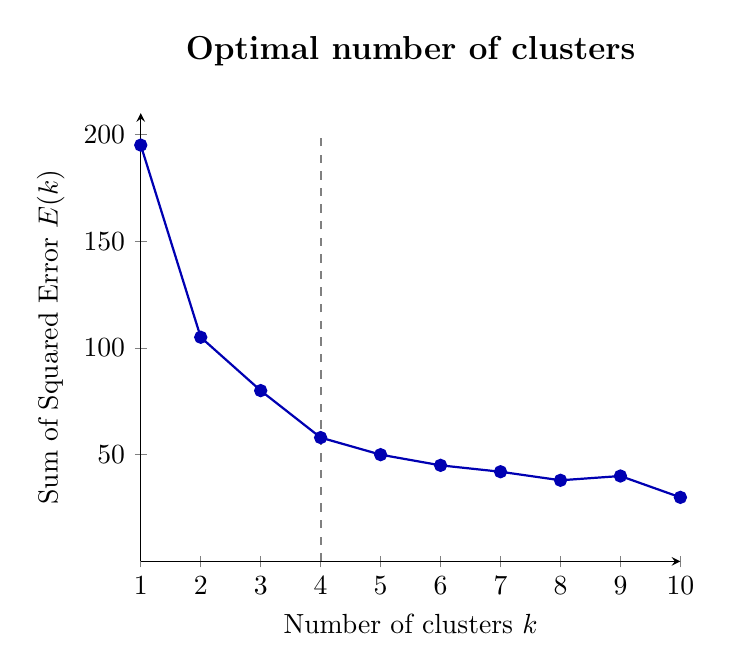
\begin{tikzpicture}
    \begin{axis}[
        title={Optimal number of clusters},
        xlabel={Number of clusters $k$},
        ylabel={Sum of Squared Error $E(k)$},
        xmin=1, xmax=10,
        ymin=0, ymax=210,
        xtick={1,2,3,4,5,6,7,8,9,10},
        ytick={50,100,150,200},
        grid=none,
        axis lines=left,
        title style={at={(0.5,1.1)}, anchor=center, font=\bfseries\large},
    ]
    % The Data Points
    \addplot[color=blue!70!black,mark=*,thick,]
    coordinates {
        (1,195) (2,105) (3,80) (4,58) (5,50) (6,45) (7,42) (8,38) (9,40) (10,30)
    };
    % The Vertical Dashed "Elbow" Line at k=4
    \draw [dashed, thick, gray] (axis cs:4,0) -- (axis cs:4,200);
    \end{axis}
    \end{tikzpicture}
    \caption{Elbow Method example plot. The elbow point is at $k=4$.}
\end{figure}
This method is really intuitive, but can be ambiguous, since the elbow point is not always clear.
For example, in the plot above, one could argue that $k=2$ or $k=3$ are also valid choices.

\subsubsection{Silhouette Method}
Increasing the number of clusters $k$ will always decrease the sum-of-squared error criterion, but it will also increase the 
similarity between different clusters. The Silhouette Method tries to balance these two aspects.
The silhouette score for a single point $x_i$ is defined as:
\begin{itemize}
    \item $a(i)$: average distance between $x_i$ and all other points in the same cluster $C$:
    \[ a(i) = \frac{1}{|C|} \sum_{j \in C} d(i, j) \]
    \item $b(i)$: minimum average distance between $x_i$ and all points in any other cluster $C'$:
    \[ b(i) = \min_{C' \neq C} \frac{1}{|C'|} d(i, C') \]
    \item The silhouette score $s(i)$ is then defined as:
    \[ s(i) = \frac{b(i) - a(i)}{\max(a(i), b(i))} \]
\end{itemize}
To choose the number of clusters $k$, we compute the average silhouette score over all points for different values of $k$. As before,
we plot the average silhouette score against $k$ and choose the value of $k$ that maximizes the score.
\begin{figure}[H]
    \centering
    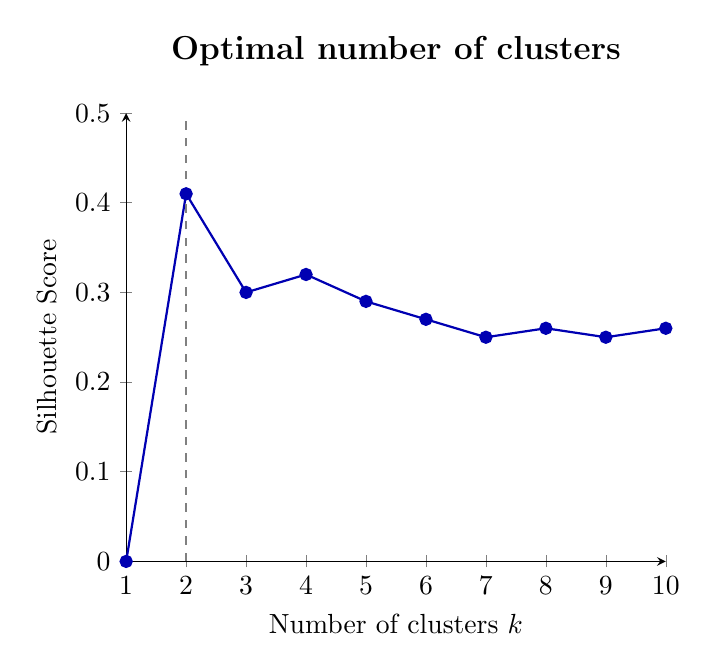
\begin{tikzpicture}
    \begin{axis}[
        title={Optimal number of clusters},
        xlabel={Number of clusters $k$},
        ylabel={Silhouette Score},
        xmin=1, xmax=10,
        ymin=0, ymax=0.5,
        xtick={1,2,3,4,5,6,7,8,9,10},
        ytick={0,0.1,0.2,0.3,0.4,0.5},
        grid=none,
        axis lines=left,
        title style={at={(0.5,1.1)}, anchor=center, font=\bfseries\large},
    ]
    % The Data Points
    \addplot[color=blue!70!black,mark=*,thick,]
    coordinates {
        (1,0.0) (2,0.41) (3,0.3) (4,0.32) (5,0.29) (6,0.27) (7,0.25) (8,0.26) (9,0.25) (10,0.26)
    };
    % The Vertical Dashed "Elbow" Line at k=4
    \draw [dashed, thick, gray] (axis cs:2,0) -- (axis cs:2,0.5);
    \end{axis}
    \end{tikzpicture}
    \caption{Silhouette Method example plot. The optimal number of clusters is at $k=2$.}
\end{figure}
\subsubsection{Hierarchical Clustering}
Hierarchical Clustering is an alternative approach, that assumes that the data is organized in a hierarchy of clusters.
This structure can be built from examples in two ways:
\begin{itemize}
    \item \textbf{Top-down approach}: start with all data points in a single cluster and recursively split clusters into smaller clusters;
    \item \textbf{Bottom-up approach}: start with each data point in its own cluster and recursively merge clusters into larger clusters.
\end{itemize}
The algorithm for the Bottom-up approach is defined as follows:
\begin{itemize}
    \item Initialize:
    \begin{itemize}
        \item Set the target number of clusters $k$;
        \item Set the initial number $\hat{k}$ of clusters to $n$;
        \item Initialize clusters as individual data points: $D_i = \{x_i\}, \forall i \in [1, n]$
    \end{itemize}
    \item Repeat until the number of clusters $\hat{k}$ is equal to $k$:
    \begin{itemize}
        \item Find the two closest clusters $D_i$ and $D_j$;
        \item Merge the clusters: $D_i \leftarrow D_i \cup D_j$;
        \item Update the number of clusters: $\hat{k} \leftarrow \hat{k} - 1$;
    \end{itemize}
\end{itemize}
The similarity between clusters can be computed in different ways:
\begin{itemize}
    \item \textbf{Nearest neighbor}: distance between the two closest points in the clusters:
    \[ d_{min}(D_i, D_j) = \min_{\boldsymbol{x} \in D_i, \boldsymbol{x'} \in D_j} ||\boldsymbol{x} - \boldsymbol{x'}|| \]
    \item \textbf{Farthest neighbor}: distance between the two farthest points in the clusters:
    \[ d_{max}(D_i, D_j) = \max_{\boldsymbol{x} \in D_i, \boldsymbol{x'} \in D_j} ||\bold{x} - \boldsymbol{x'}|| \]
    \item \textbf{Average linkage}: average distance between all points in the clusters:
    \[ d_{avg}(D_i, D_j) = \frac{1}{|D_i| |D_j|} \sum_{\boldsymbol{x} \in D_i} \sum_{\boldsymbol{x'} \in D_j} ||\boldsymbol{x} - \boldsymbol{x'}|| \]
\end{itemize}
The first two methods are sensitive to outliers, while the average linkage is more robust. All result complex to compute. A more efficient method is the \textbf{centroid method}, which computes the distance between the centroids of the clusters:
\[ d_{centroid}(D_i, D_j) = ||\mu_i - \mu_j|| \]
where $\mu_i$ and $\mu_j$ are the centroids of clusters $D_i$ and $D_j$ respectively.
